\documentclass[12pt,a4paper,oneside]{report}

\usepackage[utf8]{inputenc}
\usepackage[T1]{fontenc}
\usepackage[english]{babel}
\usepackage{lmodern}
\usepackage{microtype}
\usepackage{geometry}
\usepackage{graphicx}
% Render native SVG text in the exported PDF; this preserves draw.io line breaks.
\usepackage[inkscapeexe=/Applications/Inkscape.app/Contents/MacOS/inkscape,inkscapelatex=false]{svg}
\usepackage{placeins}
\usepackage{booktabs}
\usepackage{amsmath,amssymb}
\usepackage{titlesec}
\usepackage{hyperref}
\usepackage{csquotes}
\usepackage{array}
\usepackage[backend=biber,style=ieee]{biblatex}
\usepackage[colorinlistoftodos]{todonotes}

\geometry{margin=2.5cm}
\graphicspath{{../figures/}}
% Reusable figure template:
% \thesisfigure{file-name}{caption text}{fig:label}{0.52\textwidth}
\newcommand{\thesisfigure}[4]{%
  \begin{figure}[htbp]
    \centering
    \includegraphics[width=#4]{#1}
    \caption{#2}
    \label{#3}
  \end{figure}%
  \FloatBarrier
}

% Figure and explanatory text displayed side by side:
% \thesisfigurewithtext{file-name}{caption text}{fig:label}{explanatory text}
\newcommand{\thesisfigurewithtext}[4]{%
  \begin{figure}[htbp]
    \begin{minipage}[t]{0.48\textwidth}
      \vspace{0pt}\small #4
    \end{minipage}\hfill
    \begin{minipage}[t]{0.48\textwidth}
      \centering
      \includegraphics[width=\linewidth]{#1}
    \end{minipage}
    \caption{#2}
    \label{#3}
  \end{figure}%
}

% Keep numbered chapters, but show only their titles (without the word ``Chapter'').
\titleformat{\chapter}[display]
  {\normalfont\huge\bfseries}
  {}
  {0pt}
  {\Huge}
\addbibresource{references.bib}
\hypersetup{colorlinks=true,linkcolor=black,citecolor=black,urlcolor=blue}

\begin{document}

\begin{titlepage}
  \centering
  \vspace*{3cm}
  {\LARGE Thesis\par}
  \vspace{1.5cm}
  {\huge\bfseries Learning Latent Representations of Brain Dynamics for Modelling Alzheimer’s Disease Progression\par}
  \vfill
  {\large Author: \textit{Skaistė Butkutė}\par}
  \vspace{0.5cm}
  {\large Thesis supervisor: \textit{Pere-Pau Vázquez}\par}
  \vspace{0.5cm}
  {\large Thesis co-supervisor: \textit{Gustavo Patow}\par}
  \vspace{1.5cm}
  {\large \today\par}
\end{titlepage}

\pagenumbering{roman}
\chapter*{Abstract}
\addcontentsline{toc}{chapter}{Abstract}
% Summarise the problem, methods, main findings, and contributions here.


\chapter*{Acknowledgements}
\addcontentsline{toc}{chapter}{Acknowledgements}
% Acknowledge the people and organisations that supported this work here.


\tableofcontents
\clearpage
\pagenumbering{arabic}

\chapter{Introduction}
\section{Context and Motivation}
% Introduce Alzheimer's disease progression and the motivation for modelling brain dynamics.


\section{Objectives and Research Questions}
% State the thesis objectives and research questions.


\section{Document Structure}
% Briefly outline the remaining chapters.



\chapter{State of the Art}
\section{Alzheimer's Disease and Biomarkers}

Alzheimer’s disease (AD) has traditionally been diagnosed based on clinical symptoms, with diagnostic criteria based on progressive decline in memory and other cognitive functions~\cite{McKhann1984}. 
Mild cognitive impairment (MCI) describes a condition in which cognitive decline is present but does not significantly affect independence in daily activities~\cite{Albert2011MCI}. 
MCI can occur before dementia, but it can have different causes and does not always indicate underlying AD pathology~\cite{Albert2011MCI}. 
Therefore, clinical groups such as healthy controls (HC), MCI, and AD describe differences in cognitive and functional state rather than the underlying biological processes of the disease.

The main pathological features of AD are the accumulation of amyloid-beta (A$\beta$) and tau proteins.
A$\beta$ accumulates outside neurons and forms amyloid plaques, while abnormal tau accumulates inside neurons and forms neurofibrillary tangles~\cite{Busche2020Synergy}. 
These protein accumulations are considered key pathological features of AD\@.

A$\beta$ and tau are closely linked to the development and progression of AD\@.
Changes in these biomarkers can begin before clear cognitive symptoms appear.
A$\beta$-related changes can occur relatively early in the disease process, followed by further changes related to neuronal injury and cognitive decline.
A$\beta$ and tau are also not fully separate processes, as evidence suggests that they interact and together contribute to neuronal dysfunction~\cite{Busche2020Synergy}.
Their effects on brain activity may also differ across clinical stages.
Whole-brain modelling has shown a stronger influence of A$\beta$ on brain dynamics in MCI, while tau had a stronger influence in AD~\cite{Patow2023}.
The combination of both A$\beta$ and tau also provided a better representation of empirical brain dynamics than either biomarker individually~\cite{Patow2023}.

The use of biomarkers has led to an important distinction between the clinical diagnosis and biological definition of AD\@.
The NIA-AA Research Framework introduced the AT(N) classification system, where (A) represents A$\beta$ pathology, (T) represents tau pathology, and ((N)) represents neurodegeneration or neuronal injury~\cite{Jack2018}.
Under this framework, AD can be defined based on its underlying biological pathology rather than clinical symptoms alone~\cite{Jack2018}.
Clinical groups such as HC, MCI, and AD and biological measures of A$\beta$ and tau therefore provide different but related information.
An individual's clinical state does not always directly correspond to their biological AD status~\cite{Jack2018}.
\section{Functional Neuroimaging and Brain Connectivity}

Functional magnetic resonance imaging (fMRI) provides a non-invasive method for studying brain activity. 
It commonly measures activity through the blood-oxygen-level-dependent (BOLD) signal, which is based on changes in blood oxygenation associated with neural activity~\cite{Ogawa1990}. 
In resting-state fMRI (rs-fMRI), BOLD signals are recorded while no specific task is performed, allowing spontaneous changes in brain activity to be studied. 
Correlations between resting-state BOLD signals were first shown to identify functionally related brain regions by Biswal et al.~\cite{Biswal1995}, providing a basis for studying the functional organisation of the brain at rest.

As fMRI data contain signals across a large number of spatial locations, brain parcellation can be used to group the cortex into a smaller set of regions. 
The BOLD signal within each region can then be represented as a regional time series. 
Schaefer et al.\ proposed a cortical parcellation based on intrinsic functional connectivity, with several levels of spatial resolution ranging from 100 to 1,000 regions~\cite{Schaefer2018}.
This includes the 400-region parcellation, which provides a functionally defined representation of cortical activity.

Relationships between regional BOLD signals can be studied using functional connectivity (FC).
Functional connectivity describes statistical relationships between activity recorded from different brain regions~\cite{Friston1993}. 
In rs-fMRI, FC is commonly estimated using the Pearson correlation between pairs of regional BOLD time series~\cite{Biswal1995}. 
Calculating these correlations across the full time series produces a static FC matrix, where each value represents the strength of the functional relationship between a pair of regions. 
Static FC therefore provides a summary of functional relationships across the complete recording period.

However, functional relationships between brain regions can change over time and may not be fully represented by a single static FC matrix. 
Dynamic functional connectivity (dFC) methods study these temporal changes in connectivity~\cite{Hutchison2013}. 
A commonly used approach is sliding-window analysis, where the BOLD time series is divided into overlapping windows and an FC matrix is calculated separately for each window~\cite{Preti2017}. 
The similarity between FC patterns at different windows can then be used to describe changes in functional connectivity over time, producing a sliding-window functional connectivity dynamics (SwFCD) representation. 
This provides information about temporal changes in brain connectivity that is not captured by static FC alone~\cite{Preti2017}.

Functional connectivity can also be studied at the level of larger functional networks.
Yeo et al.\ used resting-state functional connectivity to identify large-scale organisation of the cerebral cortex and proposed parcellations consisting of seven and seventeen functional networks~\cite{Yeo2011}. 
The seven-network organisation groups cortical regions into the visual, somatomotor, dorsal attention, ventral attention, limbic, frontoparietal, and default mode networks. 
These networks provide a broader representation of functional brain organisation and can be used to interpret patterns observed across individual cortical regions.
\section{Representation Learning and Autoencoders}

Dimensionality reduction aims to represent high-dimensional data using a smaller number of features while retaining relevant information. 
A widely used linear approach is principal component analysis (PCA), originally introduced by Pearson~\cite{Pearson1901}. 
PCA transforms the input into a set of orthogonal principal components, ordered by the amount of variance they explain. 
By retaining only a subset of these components, the dimensionality of the data can be reduced while preserving as much variance as possible.

Autoencoders (AEs) provide a learned approach to dimensionality reduction. 
An autoencoder consists of an encoder that maps the input to a lower-dimensional latent representation, and a decoder that reconstructs the original input from this representation. 
The model is commonly trained by minimizing the difference between the input and its reconstruction. 
Linear autoencoders are closely related to PCA and, when trained with a squared reconstruction objective under suitable conditions, can learn the same principal subspace, although their individual latent dimensions are not required to match the principal components~\cite{BaldiHornik1989}. 
Autoencoders can also use multiple nonlinear layers, allowing them to learn more complex representations than linear dimensionality reduction. 
Hinton and Salakhutdinov demonstrated the use of deep autoencoders for reducing the dimensionality of high-dimensional data and compared their learned representations with PCA~\cite{HintonSalakhutdinov2006}.

More generally, representation learning aims to learn useful features directly from the data instead of relying on manually defined representations~\cite{Bengio2013}. 
In autoencoders, the latent space provides such a representation by compressing information needed to reconstruct the input. 
The use of nonlinear transformations and multiple layers allows deep autoencoders to capture relationships that cannot be represented by a purely linear transformation. 
The structure of this latent space can therefore provide information about how the model represents patterns present in the original high-dimensional data.

Autoencoders can also be built using convolutional layers instead of fully connected layers. 
Convolutional autoencoders apply shared filters across the input, allowing local patterns to be learned while reducing the number of independent model parameters. 
Masci et al.\ introduced stacked convolutional autoencoders for learning hierarchical representations from data~\cite{Masci2011}. 
Convolutional architectures therefore provide an alternative to fully connected autoencoders when local structure in the input may contain useful information.

A further extension is the variational autoencoder (VAE), which introduces a probabilistic latent representation. 
Rather than encoding an input directly into a single latent vector, a VAE learns the parameters of a distribution from which the latent representation is sampled. 
Kingma and Welling introduced this approach together with the reparameterization method that allows the model to be trained through standard gradient-based optimisation~\cite{KingmaWelling2014}. 
The training objective combines reconstruction with a Kullback–Leibler (KL) divergence term that regularizes the latent distribution towards a chosen prior. 
This encourages a more structured and continuous latent space while still allowing the input to be reconstructed from its lower-dimensional representation.
\section{Representation Learning of Functional Brain Dynamics}

Representation learning has been applied to functional brain data to obtain lower-dimensional descriptions of complex brain activity. 
Sanz Perl et al. used variational autoencoders (VAEs) to create low-dimensional embeddings of collective brain dynamics~\cite{SanzPerl2020}. 
Their results showed that the learned latent space can preserve meaningful differences between brain states, supporting the use of generative models for studying the organization of high-dimensional brain dynamics.

Representation learning has also been applied directly to resting-state fMRI (rs-fMRI). 
Kim et al.\ used a convolutional VAE to represent individual fMRI activity patterns in a low-dimensional latent space~\cite{Kim2021}. 
As each fMRI frame is represented separately, changes in the latent representation over time form trajectories that describe the temporal evolution of brain activity. 
The learned representations were related to patterns of cortical activity and functional connectivity, showing that information about functional brain organization can be retained after dimensionality reduction.

Low-dimensional representations can also be used to compare different global brain states. 
Sanz Perl et al.\ applied deep generative models to fMRI data from different states of consciousness and found that these states showed an ordered organization within a low-dimensional space~\cite{SanzPerl2023}. 
This demonstrates that latent-space structure can reflect differences in functional brain dynamics between conditions. 
Together, these studies show that representation learning can provide compact descriptions of high-dimensional fMRI activity while preserving information about temporal dynamics and differences between brain states.

\section{Autoencoder-Based Representation Learning in Alzheimer's Disease}
Autoencoder-based representation learning has been used to identify patterns in neuroimaging data related to Alzheimer’s disease (AD) and mild cognitive impairment (MCI). 
Early work by Suk and Shen used autoencoders to learn features from neuroimaging and biomarker data for AD/MCI classification~\cite{SukShen2013}. 
Their results showed that learned representations can contain disease-related information useful for distinguishing between clinical groups, providing an alternative to manually defined imaging features.

Autoencoders have also been applied to resting-state fMRI (rs-fMRI) to represent functional brain activity. 
Suk et al.\ used a deep autoencoder to map regional BOLD activity at individual timepoints into a lower-dimensional representation~\cite{SukStateSpace}. 
Applying the encoder across the rs-fMRI time series produced a sequence of latent representations, which was then used to model functional dynamics and distinguish individuals with MCI from healthy controls. 
Other approaches have instead learned representations from functional connectivity derived from rs-fMRI.\@ 
For example, autoencoder-based feature learning has been applied to functional brain networks for the early identification of MCI~\cite{EarlyDiagnosis2018}. 
These approaches show that disease-related information can be learned both directly from regional brain activity and from the functional relationships between brain regions.

More recent work has extended this approach towards probabilistic latent representations. 
Variational methods have been used to represent rs-fMRI functional connectivity through latent distributions for the identification of MCI~\cite{FCLatentDistributions2023}.
This allows functional connectivity patterns to be represented in a structured latent space rather than only through deterministic features. 
Overall, previous studies show that autoencoders can learn AD- and MCI-related representations from functional neuroimaging data. 
However, these representations have mainly been used as features for identifying or classifying clinical groups, with less focus on how disease-related differences are represented within the latent space and reconstructed back into functional brain activity.
\section{Longitudinal and Disease-Progression Modelling}

Longitudinal data provide information about how Alzheimer’s disease (AD) develops over time by following individuals across multiple clinical visits. 
While cross-sectional studies can identify differences between clinical groups at a particular point in time, longitudinal measurements allow changes within individuals to be studied. 
Representation learning methods can use these repeated measurements to learn disease-related changes and trajectories of progression.

Yang et al.\ proposed a sequential graph autoencoder for modelling longitudinal neuroimaging data in preclinical AD~\cite{Yang2021}. The model combines relationships between brain regions with information from repeated clinical visits and separates the latent representation into time-varying and time-invariant components. 
The time-varying representation captures changes across visits, while the time-invariant representation captures characteristics that remain relatively stable over time. 
This demonstrates how autoencoder-based representations can be structured to distinguish longitudinal disease-related changes from more stable subject-specific information.

Longitudinal progression has also been modelled using recurrent variational autoencoders. 
Martí-Juan et al.\ proposed a multi-channel recurrent variational autoencoder (MC-RVAE) for modelling multimodal AD progression~\cite{MartiJuan2023}. 
The model uses a shared latent representation to capture relationships between different data modalities while recurrent components model their changes over time. 
This allows longitudinal trajectories to be reconstructed and missing measurements to be estimated, demonstrating how generative latent-variable models can represent the temporal progression of multiple AD-related measurements.

Disease progression can also be represented as a continuous trajectory within a learned latent space. 
Hong et al.\ used a variational autoencoder to learn representations of tau PET images and derive a pseudo-temporal trajectory describing the progression of tau pathology~\cite{Hong2022}. 
The resulting trajectory reflected changes in the spatial distribution of tau and was associated with clinical and biological measures of AD.\@ 
Together, these studies show that learned representations can be used not only to distinguish clinical groups, but also to describe disease-related changes over time and represent progression as a continuous process.

\section{Brain Connectivity Representation and Translation}

Learned representations of brain activity can be used not only for dimensionality reduction, but also to study how latent dimensions relate to functional brain organisation. 
Sanz Perl et al.\ used a variational autoencoder to obtain low-dimensional representations of parcellated fMRI activity~\cite{SanzPerl2025}. 
Individual latent dimensions were perturbed and decoded back into regional brain activity, allowing their spatial patterns to be related to large-scale functional networks. 
This showed that information represented within individual latent dimensions can be mapped back to interpretable patterns of functional brain organisation.

Latent representations can also provide a common space for translating between different representations of brain connectivity. 
Jamison et al.\ proposed Krakencoder, an encoder-decoder framework that maps different structural and functional connectomes into a shared latent representation~\cite{Jamison2025}. 
Separate encoders and decoders are used for different connectivity representations, allowing one representation to be encoded into the shared space and reconstructed as another. 
This demonstrates how a common latent representation can be combined with different decoders to reconstruct or translate between related representations of brain organisation.

Shared representations of structural and functional connectivity have also been investigated in relation to Alzheimer’s disease. 
Amodeo et al.\ proposed a graph variational autoencoder that combines structural connectivity with resting-state functional connectivity within a joint latent representation~\cite{Amodeo2022}. 
The learned representations were evaluated using data from the OASIS-3 dataset and contained information relevant to distinguishing AD-related populations. 
Together, these studies show that latent representations can preserve information about functional brain organisation, provide interpretable mappings back to brain networks, and support translation between different brain representations. 
These approaches provide a basis for investigating whether a shared representation can also be decoded into different disease-related functional brain states.


\chapter{Methodology}
\section{Data and Preprocessing}

The data were obtained from the Alzheimer's Disease Neuroimaging
Initiative (ADNI)~\cite{ADNI}. Two datasets were used: a primary dataset
(\textbf{ADNI-B}) and a longitudinal dataset (\textbf{ADNI-Long}).
Both contain resting-state functional magnetic resonance imaging
(rs-fMRI), regional amyloid-$\beta$ (A$\beta$) and tau measurements,
and a clinical diagnosis for each session. Diagnoses were grouped as
healthy controls (HC), mild cognitive impairment (MCI), and Alzheimer's
disease (AD).

ADNI-B contains 152 ADNI3 participants, with one session per
participant. It was used for model development and evaluation.
ADNI-Long contains data from ADNI1, ADNIGO, ADNI2, and ADNI3. Before
longitudinal selection, it included 141 participants and 281 sessions.
Its repeated sessions allow changes in clinical stage to be studied
across visits.

Both datasets were provided in preprocessed and parcellated form.
Neuroimaging preprocessing, denoising, spatial normalisation, temporal
filtering, and brain parcellation were therefore not performed in this
work. The datasets were processed independently using the same
procedure, so matching sessions are not necessarily numerically
identical. Sections~\ref{sec:neuroimaging_preprocessing}
and~\ref{sec:dataset_consistency} describe the upstream procedure and
the comparison between datasets, respectively.


\subsection{Sample Selection and Cohort Characteristics}
\label{sec:sample_selection}

ADNI-B was the cross-sectional cohort for training, validation, and
testing. Its 152 samples represent different participants: 93 HC, 33
MCI, and 26 AD.

ADNI-Long was used to evaluate changes associated with clinical
progression. Participants with unchanged diagnoses across all available
visits were excluded because the analysis focuses on changes between
clinical stages. Transitions to an earlier stage were also excluded.
The selected cohort therefore represents forward progression between
HC, MCI, and AD rather than all trajectories in ADNI-Long.

Participants with three sessions and different diagnoses were split
into pairs representing clinical progression. The construction of these
pairs is described in Section~\ref{sec:longitudinal_construction}.

Participants shared by the selected ADNI-Long cohort and ADNI-B were
identified. To avoid subject-level information leakage, their ADNI-B
samples were assigned only to the test set. They were therefore not
included in the training or validation data.

Table~\ref{tab:dataset_summary} summarises ADNI-B, the available
ADNI-Long dataset, and the selected longitudinal cohort.

\begin{table}[ht]
    \centering
    \caption{Summary of the available and selected datasets. Diagnostic
    counts for ADNI-Long are reported at the session level.}
    \label{tab:dataset_summary}
    \begin{tabular}{lccc}
        \hline
        & ADNI-B & ADNI-Long Available & ADNI-Long Selected \\
        \hline
        ADNI phases & ADNI3 & ADNI1/GO/2/3 & ADNI1/2/3 \\
        Unique subjects & 152 & 141 & 22 \\
        Sessions & 152 & 281 & 48 \\
        HC sessions & 93 & 175 & 15 \\
        MCI sessions & 33 & 76 & 23 \\
        AD sessions & 26 & 30 & 10 \\
        \hline
    \end{tabular}
\end{table}

Table~\ref{tab:demographics} shows the demographic characteristics of
the final cohorts. Mean age was similar across groups in ADNI-B
(73.26--75.88 years) and ADNI-Long (73.87--74.67 years). Sex was also
relatively balanced, although the AD group in ADNI-B contained more
males (61.5\%).

ADNI-Long characteristics are reported at the session level. A
participant may therefore contribute to more than one clinical group as
their diagnosis changes across visits.

\begin{table}[ht]
    \centering
    \caption{Demographic characteristics of the final ADNI-B and selected
    ADNI-Long cohorts. Age is reported as mean $\pm$ standard deviation.
    ADNI-Long characteristics are reported at the session level.}
    \label{tab:demographics}
    \begin{tabular}{llcccc}
        \hline
        Dataset & Group & N & Age (years) & Female, n (\%) & Male, n (\%) \\
        \hline
        ADNI-B
            & HC  & 93 & $73.26 \pm 5.33$ & 48 (51.6\%) & 45 (48.4\%) \\
            & MCI & 33 & $73.72 \pm 6.37$ & 19 (57.6\%) & 14 (42.4\%) \\
            & AD  & 26 & $75.88 \pm 7.51$ & 10 (38.5\%) & 16 (61.5\%) \\
        \hline
        ADNI-Long
            & HC  & 15 & $74.65 \pm 5.03$ & 6 (40.0\%) & 9 (60.0\%) \\
            & MCI & 23 & $74.67 \pm 6.64$ & 11 (47.8\%) & 12 (52.2\%) \\
            & AD  & 10 & $73.87 \pm 6.85$ & 4 (40.0\%) & 6 (60.0\%) \\
        \hline
    \end{tabular}
\end{table}

\subsection{Upstream Neuroimaging Preprocessing}
\label{sec:neuroimaging_preprocessing}

The neuroimaging data were preprocessed before they were provided.
This section describes that upstream preparation, not preprocessing
performed in this thesis.

Functional MRI preprocessing used the standard volume-based CONN
pipeline. It included realignment and motion correction, slice-timing
correction, and outlier detection with the Artifact Detection Toolbox
(ART). Functional images were coregistered to each participant's
high-resolution T1-weighted image and normalised to MNI-152 space with
2~mm isotropic resampling. They were then smoothed with an 8~mm FWHM
Gaussian kernel~\cite{AquileLlorensMartinezMolina}.

Denoising used anatomical CompCor (aCompCor)~\cite{Behzadi2007}. Five
principal components from white matter and five from cerebrospinal
fluid were regressed from the functional data. Nuisance regressors also
included six realignment parameters, their first-order temporal
derivatives, and ART-identified artifacts. The denoised BOLD time
series were band-pass filtered between 0.008 and
0.08~Hz~\cite{AquileLlorensMartinezMolina}.

ADNI-B and ADNI-Long underwent the same procedure but were processed
independently. Section~\ref{sec:dataset_consistency} examines the
effect on the parcellated BOLD signals.


\subsection{Brain Parcellation and BOLD Representation}
\label{sec:bold_representation}

During upstream preparation, the functional data were parcellated with
the 400-region Schaefer cortical atlas~\cite{Schaefer2018}. The
provided data therefore contain regional BOLD time series rather than
voxel-level fMRI volumes.

Each parcel is represented by one BOLD time series. An rs-fMRI sample
is represented as

\begin{equation}
    \mathbf{X} \in \mathbb{R}^{R \times T},
\end{equation}

where $R=400$ is the number of cortical regions and $T=197$ is the
number of timepoints. Each element $x_{r,t}$ is the BOLD signal for
region $r$ at timepoint $t$. Each session is thus a
$400 \times 197$ matrix.

% The 400 parcels can also be assigned to the seven large-scale networks
% described by Yeo et al.~\cite{Yeo2011}. These assignments are not model
% inputs. They are used later to interpret learned representations in
% terms of large-scale brain organisation.

Figure~\ref{fig:bold_example} shows an example of the parcellated BOLD
representation used as input to the models.

\begin{figure}[ht]
    \centering
    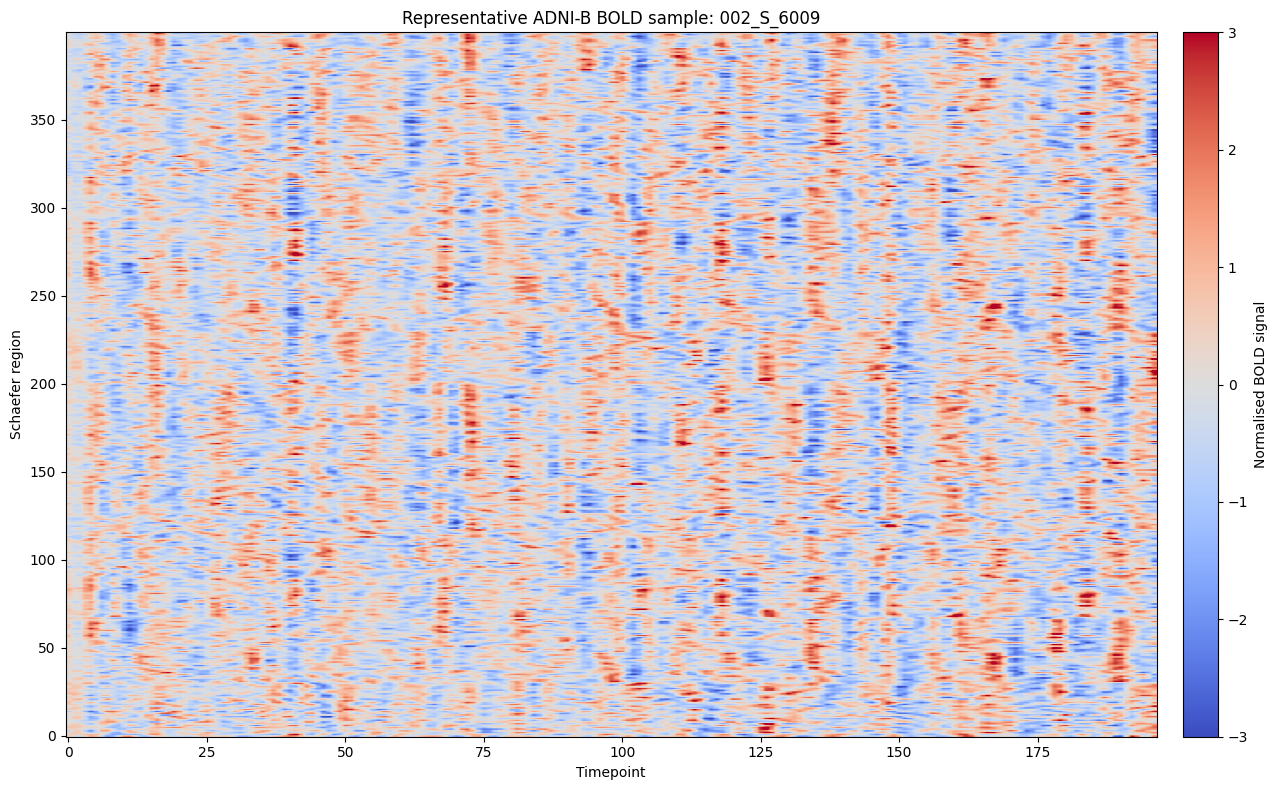
\includegraphics[width=0.85\textwidth]
    {example_bold_heatmap.png}
    \caption{Example parcellated rs-fMRI sample used as input to the
    models. Each row represents one of the 400 Schaefer cortical
    parcels and each column represents one of the 197 available
    timepoints.}
    \label{fig:bold_example}
\end{figure}


\subsection{Amyloid-$\beta$ and Tau Data}
\label{sec:biomarker_data}

The A$\beta$ and tau PET data were also provided after preprocessing
and parcellation. The following PET steps were performed upstream.

PET images were coregistered to the corresponding T1-weighted image and
smoothed to 8~mm FWHM. Partial-volume correction used the
Müller--Gärtner method in PETPVC~\cite{Thomas2016}.

A$\beta$ measurements came from Florbetapir (FBP) or Florbetaben (FBB)
PET scans. Standardized Uptake Value Ratios (SUVRs) used the whole
cerebellum as the reference region and were converted to Centiloid
units with tracer-specific calibration equations. Tau measurements came
from Flortaucipir PET scans. Their SUVRs used inferior cerebellar grey
matter as the reference region~\cite{AquileLlorensMartinezMolina}.

The upstream procedure parcellated PET data with the Schaefer-400
atlas. Each session is associated with regional A$\beta$ and tau
vectors,

\begin{equation}
    \mathbf{a} \in \mathbb{R}^{400},
    \qquad
    \boldsymbol{\tau} \in \mathbb{R}^{400},
\end{equation}

where $a_r$ and $\tau_r$ are the A$\beta$ and tau measurements for
region $r$.


\subsection{Input Normalisation}
\label{sec:input_normalisation}

Further normalisation was performed before the data were passed to the
models. BOLD time series and regional A$\beta$ and tau measurements
used different procedures.

Each regional BOLD time series was standardised across time using a
z-score,

\begin{equation}
    \tilde{x}_{r,t}
    =
    \frac{x_{r,t}-\mu_r}{\sigma_r},
\end{equation}

where $\mu_r$ and $\sigma_r$ are the temporal mean and standard
deviation of region $r$ in that session. This was done independently
for every region and session. It removes differences in signal scale
while preserving temporal fluctuations. Each normalised time series has
zero temporal mean and unit temporal standard deviation. The same
procedure was used for ADNI-B and ADNI-Long.

A$\beta$ and tau were instead normalised across subjects. For each
biomarker and region, the mean and standard deviation were calculated
from the ADNI-B training set only. A regional biomarker value $b_r$ was
then standardised as

\begin{equation}
    \tilde{b}_{r}
    =
    \frac{b_{r}-\mu_{r}^{\mathrm{train}}}
         {\sigma_{r}^{\mathrm{train}}},
\end{equation}

where $b_r$ is the A$\beta$ or tau value for region $r$.
$\mu_{r}^{\mathrm{train}}$ and $\sigma_{r}^{\mathrm{train}}$ are the
corresponding mean and standard deviation across training subjects.
This was done separately for each of the 400 regions and for each
biomarker.

The ADNI-B training statistics were used to normalise the validation
and test sets. They were also used for ADNI-Long when evaluating models
developed on ADNI-B. This prevents validation, test, and longitudinal
data from influencing model development.


\subsection{Consistency Between ADNI-B and ADNI-Long}
\label{sec:dataset_consistency}

Although ADNI-B and ADNI-Long underwent the same upstream neuroimaging
preprocessing procedure, the datasets were processed independently.
Consequently, sessions corresponding to the same participant and
acquisition are not numerically identical between the two datasets.
Since models developed using ADNI-B are subsequently evaluated using
longitudinal observations from ADNI-Long, the consistency between the
independently processed datasets was assessed before longitudinal
evaluation.

Sessions corresponding to the same participant and acquisition were
identified in both datasets and compared at three levels: regional BOLD
activity, static functional connectivity (FC), and sliding-window
functional connectivity dynamics (SwFCD). These comparisons were used
to determine whether differences introduced by the independent
processing affected the regional signals themselves, their static
functional relationships, or their temporal connectivity structure.

For each matched session, the normalised BOLD matrices from ADNI-B and
ADNI-Long were flattened into vectors containing all cortical regions
and timepoints,

\begin{equation}
    \mathbf{x}^{B}
    =
    \operatorname{vec}(\mathbf{X}^{B}),
    \qquad
    \mathbf{x}^{Long}
    =
    \operatorname{vec}(\mathbf{X}^{Long}),
\end{equation}

where
$\mathbf{x}^{B},\mathbf{x}^{Long}\in\mathbb{R}^{RT}$,
with $R=400$ regions and $T=197$ timepoints. Each vector therefore
contains $78{,}800$ corresponding normalised BOLD values. Similarity
between the two BOLD representations was calculated using Pearson
correlation,

\begin{equation}
    \rho_{\mathrm{BOLD}}
    =
    \operatorname{corr}
    \left(
        \mathbf{x}^{B},
        \mathbf{x}^{Long}
    \right).
\end{equation}

Static FC was calculated from the Pearson correlation between every
pair of regional BOLD time series. The unique off-diagonal elements of
the resulting FC matrices were vectorised, and similarity between the
two datasets was calculated as

\begin{equation}
    \rho_{\mathrm{FC}}
    =
    \operatorname{corr}
    \left(
        \operatorname{vec}_{u}(\mathbf{FC}^{B}),
        \operatorname{vec}_{u}(\mathbf{FC}^{Long})
    \right),
\end{equation}

where $\operatorname{vec}_{u}$ denotes vectorisation of the upper
triangular elements of a matrix, excluding the diagonal.

SwFCD was compared in the same manner using the unique off-diagonal
elements of the corresponding SwFCD matrices,

\begin{equation}
    \rho_{\mathrm{SwFCD}}
    =
    \operatorname{corr}
    \left(
        \operatorname{vec}_{u}(\mathbf{SwFCD}^{B}),
        \operatorname{vec}_{u}(\mathbf{SwFCD}^{Long})
    \right).
\end{equation}

In addition to Pearson correlation, mean absolute error (MAE) was used
to quantify the numerical difference between corresponding values. For
two vectorised representations $\mathbf{u}$ and $\mathbf{v}$ containing
$N$ corresponding elements, MAE was calculated as

\begin{equation}
    \mathrm{MAE}(\mathbf{u},\mathbf{v})
    =
    \frac{1}{N}
    \sum_{i=1}^{N}
    \left|u_i-v_i\right|.
\end{equation}

For BOLD, MAE was therefore calculated across the $78{,}800$
corresponding region--timepoint values. For FC and SwFCD, it was
calculated across the corresponding vectorised upper-triangular
elements. Pearson correlation and MAE provide complementary measures:
Pearson correlation evaluates similarity in the relative structure of
the representations, whereas MAE measures the magnitude of their
pointwise numerical differences.

Figure~\ref{fig:dataset_consistency_example} shows a representative
comparison of the BOLD, FC, and SwFCD representations from a session
present in both datasets.

\begin{figure}[ht]
    \centering
    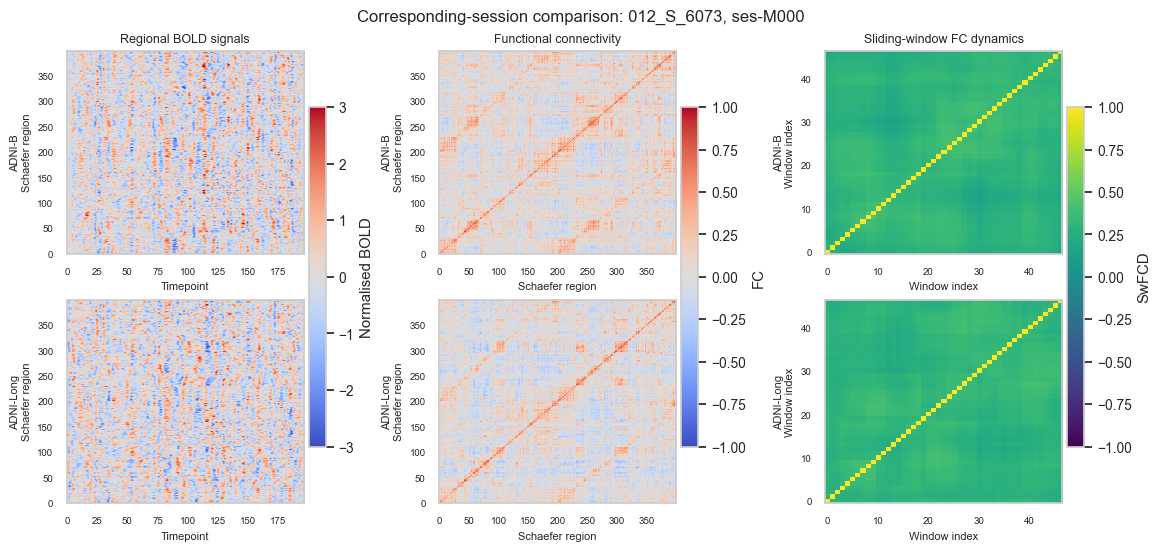
\includegraphics[width=\textwidth]
    {b2_long_comparison.png}
    \caption{Representative comparison of a session present in both
    ADNI-B and ADNI-Long. The columns show the corresponding normalised
    regional BOLD signals, static functional connectivity (FC), and
    sliding-window functional connectivity dynamics (SwFCD). The upper
    row represents ADNI-B and the lower row represents ADNI-Long.}
    \label{fig:dataset_consistency_example}
\end{figure}

A total of eight sessions could be matched between ADNI-B and
ADNI-Long. The same BOLD, FC, and SwFCD comparisons were performed for
each shared session to assess whether the observed consistency extended
beyond an individual example. The resulting Pearson correlations and
MAE values are shown in
Figure~\ref{fig:dataset_consistency_population}.

\begin{figure}[ht]
    \centering
    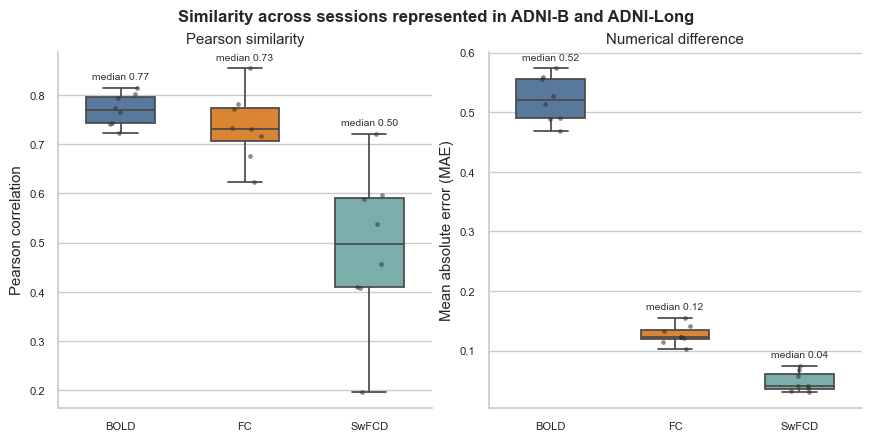
\includegraphics[width=\textwidth]
    {dataset_consistency_population.png}
    \caption{Consistency between the eight sessions represented in both
    ADNI-B and ADNI-Long. Boxplots show the Pearson correlation and mean
    absolute error (MAE) between corresponding BOLD, FC, and SwFCD
    representations. Individual points represent shared sessions, and
    annotations indicate the median across sessions.}
    \label{fig:dataset_consistency_population}
\end{figure}

Across the eight shared sessions, the mean Pearson correlations were
0.770 for BOLD, 0.736 for FC, and 0.490 for SwFCD. The corresponding
mean MAE values were 0.522, 0.126, and 0.047, respectively. BOLD and FC
showed reasonably consistent correlations across the shared sessions,
indicating that their overall signal and static connectivity structure
was largely preserved between the independently processed datasets.

SwFCD showed lower and more variable Pearson correlations, indicating
that its relative structure was less consistently preserved. Within
the SwFCD representation, however, the corresponding absolute
differences remained relatively small, with a mean MAE of 0.047. This
difference between the Pearson correlation and MAE results demonstrates
that small pointwise numerical differences can coexist with weaker
preservation of the relative structure of a representation.

Overall, the independently processed datasets should not be considered
numerically equivalent. Nevertheless, the consistency check indicates
that the BOLD and static FC representations retained a reasonable degree
of similarity across the shared sessions, while larger differences were
observed in the relative structure of SwFCD. Since only eight sessions
were available in both datasets, these results are interpreted as a
dataset consistency check rather than as evidence of equivalence between
ADNI-B and ADNI-Long.

\subsection{Longitudinal Dataset Construction}
\label{sec:longitudinal_construction}

After the selection described in Section~\ref{sec:sample_selection},
the remaining ADNI-Long sessions were organised into longitudinal
pairs. Each pair contains a source and target observation from the same
participant at different visits,

\begin{equation}
    \left(
        \mathbf{X}_{t_1},
        \mathbf{X}_{t_2}
    \right),
    \qquad t_1 < t_2,
\end{equation}

where $\mathbf{X}_{t_1}$ is the source state and
$\mathbf{X}_{t_2}$ is the target state. The source session is the
earlier visit and the target session is the later visit. Their clinical
labels are referred to as the source diagnosis and target diagnosis,
respectively.

Only forward transitions between different clinical groups were kept:
HC~$\rightarrow$~MCI, HC~$\rightarrow$~AD, and
MCI~$\rightarrow$~AD. Stable and reverse transitions were excluded.

For participants with more than two sessions, all temporally ordered
source--target pairs representing valid forward transitions were
retained. A session could therefore contribute to more than one pair.
For example, for a participant with three chronologically ordered
diagnoses

\begin{equation}
    \left[
        \mathrm{MCI}_{t_1},
        \mathrm{AD}_{t_2},
        \mathrm{AD}_{t_3}
    \right],
    \qquad t_1 < t_2 < t_3,
\end{equation}

the resulting source--target pairs are

\begin{equation}
    \left(
        \mathrm{MCI}_{t_1},
        \mathrm{AD}_{t_2}
    \right)
    \quad \text{and} \quad
    \left(
        \mathrm{MCI}_{t_1},
        \mathrm{AD}_{t_3}
    \right).
\end{equation}

The pair $\left(\mathrm{AD}_{t_2},\mathrm{AD}_{t_3}\right)$ is excluded
because the diagnosis does not change. More generally, every temporally ordered source--target combination
representing one of the valid forward transitions
HC~$\rightarrow$~MCI, HC~$\rightarrow$~AD, or
MCI~$\rightarrow$~AD is retained. This allows several
progression intervals from one participant while excluding stable and
reverse transitions.

The selected ADNI-Long cohort contains 22 participants and 48 sessions,
which produced 27 progression pairs. Participants and sessions can
contribute to more than one pair or transition type.
Table~\ref{tab:longitudinal_transitions} summarises these pairs.

\begin{table}[ht]
    \centering
    \caption{Clinical progression pairs represented in the selected
    ADNI-Long cohort. The number of unique subjects within each
    transition type is not additive because the same participant may
    contribute to more than one type of clinical transition.}
    \label{tab:longitudinal_transitions}
    \begin{tabular}{lcc}
        \hline
        Transition & Unique subjects & Pairs \\
        \hline
        HC $\rightarrow$ MCI & 13 & 15 \\
        HC $\rightarrow$ AD  & 1  & 1  \\
        MCI $\rightarrow$ AD & 10 & 11 \\
        \hline
        Total & 22 & 27 \\
        \hline
    \end{tabular}
\end{table}

The interval between the source and target sessions was recorded for
each pair to describe the period over which the transition was observed.
Across the 27 longitudinal pairs, the mean interval was $2.90 \pm 1.05$ years.

As described in Section~\ref{sec:sample_selection}, participants shared
by ADNI-Long and ADNI-B were restricted to the ADNI-B test set. Thus,
longitudinal participants did not contribute to training or validation.

\section{Autoencoder Framework}

Autoencoders were used to learn compact representations of preprocessed
resting-state fMRI BOLD signals while reconstructing the original data.
As described in Section~\ref{sec:bold_representation}, each session is
represented by a parcellated BOLD time series,
\[
\mathbf{X} \in \mathbb{R}^{T \times R},
\]
where $T$ is the number of timepoints and $R$ is the number of brain
regions. The models operate directly on this representation, rather than
on connectivity matrices or other features derived from it.

An autoencoder has an encoder and a decoder. The encoder $f_{\theta}$
maps the input to a lower-dimensional latent representation,
\[
\mathbf{Z} = f_{\theta}(\mathbf{X}),
\]
where $\mathbf{Z}$ is the compressed representation. The decoder
$g_{\phi}$ maps this representation back to the input space,
\[
\hat{\mathbf{X}} = g_{\phi}(\mathbf{Z}),
\]
where $\hat{\mathbf{X}}$ is the reconstructed BOLD time series. The
complete mapping is
\[
\hat{\mathbf{X}} = g_{\phi}\left(f_{\theta}(\mathbf{X})\right).
\]

The latent representation is an information bottleneck. The models
compress the regional dimension from $R$ to $L$, where $L<R$, while
preserving the temporal dimension. Thus,
\[
\mathbf{X} \in \mathbb{R}^{T \times R}
\longrightarrow
\mathbf{Z} \in \mathbb{R}^{T \times L}
\longrightarrow
\hat{\mathbf{X}} \in \mathbb{R}^{T \times R}.
\]

Each latent feature therefore has a time-dependent trajectory across the scan. The representation describes regional BOLD activity at every timepoint in a lower-dimensional space.
This framework was used for linear, deep fully connected, and convolutional autoencoders. The architectures differ in their encoder and decoder transformations but share the same time-preserving latent format and the common objective of reconstructing the input BOLD signal.

\subsection{Linear Autoencoder}
\thesisfigure{architectures/linearAE}{Linear autoencoder architecture diagram}{fig:lae_diagram}{0.8\textwidth}

The linear autoencoder is the simplest architecture considered. As shown
in Figure~\ref{fig:lae_diagram}, it has one linear encoder layer and one
linear decoder layer. Given an input BOLD time series
\[
\mathbf{X}\in\mathbb{R}^{T\times R},
\]
the encoder maps regional activity at each timepoint from $R$ dimensions
to $L$ dimensions,
\[
\mathbf{X}\in\mathbb{R}^{T\times R}
\longrightarrow
\mathbf{Z}\in\mathbb{R}^{T\times L}.
\]

For each time point $t$, the encoding operation is given by
\[
\mathbf{z}_t = \mathbf{W}_e\mathbf{x}_t + \mathbf{b}_e,
\]
where $\mathbf{x}_t\in\mathbb{R}^{R}$ is regional BOLD activity at
timepoint $t$, $\mathbf{W}_e\in\mathbb{R}^{L\times R}$ is the encoder
weight matrix, and $\mathbf{b}_e\in\mathbb{R}^{L}$ is its bias vector.

The same encoder parameters are applied independently at every
timepoint. This preserves the temporal dimension and makes the number of
trainable parameters independent of $T$.

The decoder maps the latent representation back to the original regional dimensionality,
\[
\hat{\mathbf{x}}_t = \mathbf{W}_d\mathbf{z}_t + \mathbf{b}_d,
\]
where $\mathbf{W}_d\in\mathbb{R}^{R\times L}$ and
$\mathbf{b}_d\in\mathbb{R}^{R}$. Applying the decoder at all timepoints
restores the original dimensionality,
\[
\mathbf{Z}\in\mathbb{R}^{T\times L}
\longrightarrow
\hat{\mathbf{X}}\in\mathbb{R}^{T\times R}.
\]

No nonlinear activation is used. The model therefore learns a
low-dimensional linear representation of regional BOLD activity. Because
each timepoint is processed independently, it does not explicitly model
temporal interactions.

For $R$ input regions and $L$ latent dimensions, the encoder has
$RL+L$ trainable parameters and the decoder has $LR+R$. The total is
$2RL+L+R$.

\subsection{Deep Autoencoder}
\thesisfigure{architectures/deepAE}{Deep autoencoder architecture diagram}{fig:dae_diagram}{\textwidth}

The deep autoencoder extends the linear model with one or two nonlinear
hidden layers before the latent bottleneck. The decoder has the mirrored
structure. Figure~\ref{fig:dae_diagram} shows the evaluated
configurations.

For a single hidden layer, the architecture is
\[
(T,R)\rightarrow(T,H_1)\rightarrow(T,L)\rightarrow(T,H_1)\rightarrow(T,R),
\]
while the two-hidden-layer configuration is
\[
(T,R)\rightarrow(T,H_1)\rightarrow(T,H_2)\rightarrow(T,L)
\rightarrow(T,H_2)\rightarrow(T,H_1)\rightarrow(T,R).
\]

The hidden dimensions $H_1$ and $H_2$ determine the width of the
nonlinear mappings, while $L$ determines the bottleneck size. Hidden
linear layers use GELU activations. The latent projection and final
reconstruction layer remain linear.

As in the linear autoencoder, the same transformations are applied
independently at each timepoint. The temporal dimension is preserved,
but dependencies between neighbouring timepoints are not modelled
explicitly.

The composition of linear transformations and GELU activations allows the
encoder and decoder to learn nonlinear mappings between the regional and
latent representations, increasing representational capacity relative to
the linear autoencoder. Each encoder hidden layer has a corresponding decoder layer.

The experiments used one or two hidden layers to limit model complexity
and computational cost. The latent and hidden-layer dimensions were
varied as architectural hyperparameters.




\subsection{Convolutional Autoencoder}

\subsubsection{Two-Dimensional Convolutional Autoencoder}
\thesisfigure{architectures/conv2dAE}{Conceptual 2D convolutional autoencoder architecture diagram}{fig:conv2dae_diagram}{\textwidth}

The two-dimensional convolutional autoencoder applies convolutions
across the temporal and regional dimensions of the BOLD signal. Its
conceptual architecture is shown in Figure~\ref{fig:conv2dae_diagram}.

The model was motivated by convolutional approaches to neuroimaging
representation learning. It was designed to test whether local features
across time and regional parcel indices improve the learned
representation while retaining a time-preserving latent space.

The architecture preserves the time dimension while reducing the regional
dimension from $R$ to $L$. It therefore produces
$\mathbf{Z}\in\mathbb{R}^{T\times L}$ rather than compressing the whole
scan into one feature map.

The input BOLD signal is represented as
\[
\mathbf{X}\in\mathbb{R}^{T\times R}.
\]
For two-dimensional convolutions, a singleton channel dimension is added,
\[
(B,T,R)\rightarrow(B,1,T,R),
\]
where $B$ is the batch size.

The encoder can contain zero, one, or two hidden convolutional layers.
Each hidden layer applies a two-dimensional convolution and GELU
activation,
\[
\mathbf{H}^{(i)}
=
\operatorname{GELU}
\left(
\operatorname{Conv2D}
\left(
\mathbf{H}^{(i-1)}
\right)
\right).
\]
The kernels extend across time and regions, so a representation can use
neighbouring temporal observations. The temporal stride is one, which
preserves the number of timepoints.

For consistency across architectures, $H_1$ and $H_2$ denote hidden-layer
sizes. In the fully connected architecture, they represent hidden feature
dimensions. In the convolutional architectures, they represent the
number of feature channels. Thus, the 2D hidden convolutional layers
produce $H_1$ and, where used, $H_2$ channels, while $L$ denotes the
width of the final bottleneck.

After the optional hidden layers, a depthwise convolution reduces the
regional dimension. Its kernel and stride operate only along the
regional axis; both are one along the temporal axis. Conceptually,
\[
(H,T,R')
\rightarrow
(H,T,L),
\]
where $R'$ is the regional width after hidden convolutions and $H$ is the
number of channels. Depthwise convolution processes each channel
independently.

A subsequent $1\times1$ convolution combines the feature channels into
one latent channel without changing the temporal or regional dimensions.
The resulting representation is
\[
\mathbf{Z}\in\mathbb{R}^{T\times L}.
\]
This gives one $L$-dimensional vector at each timepoint. The model
reshapes tensors between the convolutional layout and
$\mathbf{Z}\in\mathbb{R}^{T\times L}$ as required.

The decoder reverses this process. A $1\times1$ convolution expands the
latent representation to the required number of channels, and a
depthwise transposed convolution restores regional width. Hidden
convolutional layers are reversed in order. Intermediate decoder layers
use GELU activations and the final layer is linear. The output is
reshaped to
\[
\hat{\mathbf{X}}\in\mathbb{R}^{T\times R}.
\]

Unlike the fully connected models, this architecture uses local temporal
context without reducing temporal resolution. Along the regional axis,
convolution uses neighbouring Schaefer parcel indices, which do not
necessarily represent anatomically adjacent regions. The model therefore
learns local temporal--regional-index patterns rather than explicit
anatomical neighbourhoods.

The experiments considered zero, one, or two hidden convolutional
layers. The latent dimensionality, number of hidden layers, and channel
dimensions were architectural hyperparameters.

\subsubsection{One-Dimensional Regional Convolutional Autoencoder}
\thesisfigure{architectures/convAE}{Conceptual 1D convolutional autoencoder architecture diagram}{fig:convae_diagram}{\textwidth}

The one-dimensional convolutional autoencoder is an intermediate model
between timepoint-wise fully connected autoencoders and the
two-dimensional convolutional model. It tests regional convolution
without temporal convolution. It was introduced to determine whether
regional convolutional feature extraction improves representation
learning independently of temporal convolution.
Figure~\ref{fig:convae_diagram} shows the conceptual architecture.

As with the linear and deep models, each timepoint is processed
independently with shared encoder and decoder parameters. The input
tensor
\[
\mathbf{X}\in\mathbb{R}^{B\times T\times R}
\]
is internally reshaped to
\[
(BT,1,R),
\]
so that each timepoint is an independent one-dimensional regional signal.
The convolutions operate only along the regional axis. After encoding,
the representation is reshaped to
\[
\mathbf{Z}\in\mathbb{R}^{B\times T\times L},
\]
which preserves one $L$-dimensional vector for every timepoint.

The encoder can contain zero, one, or two hidden convolutional layers.
Each hidden layer applies a one-dimensional convolution and GELU
activation,
\[
\mathbf{H}^{(i)}
=
\operatorname{GELU}
\left(
\operatorname{Conv1D}
\left(
\mathbf{H}^{(i-1)}
\right)
\right).
\]
The hidden-layer sizes $H_1$ and $H_2$ denote the number of channels in
their respective convolutional layers. Together with the number of
hidden layers, they control feature-extractor capacity. The latent
dimensionality $L$ determines bottleneck size.

After optional hidden feature extraction, a depthwise one-dimensional
convolution reduces regional width from $R$ to $L$ while processing each
channel independently,
\[
(BT,H,R)\rightarrow(BT,H,L),
\]
where $H$ is the number of channels. The reduction-layer kernel and
stride are selected to give exactly $L$ output positions.

A $1\times1$ convolution then combines the feature channels without
changing regional width,
\[
(BT,H,L)\rightarrow(BT,1,L).
\]
After removing the channel dimension and restoring batch and temporal
dimensions, this gives
\[
\mathbf{Z}\in\mathbb{R}^{B\times T\times L}.
\]
The latent representation at timepoint $t$ therefore depends only on the
regional BOLD values at that timepoint,
\[
\mathbf{z}_t=f_{\theta}(\mathbf{x}_t),
\]
and not on neighbouring observations.

The decoder reverses this process. A $1\times1$ convolution expands the
latent representation to the required number of channels, and a
depthwise transposed convolution restores the regional dimension from
$L$ to $R$. Hidden layers are reversed to return to one output channel.
Intermediate layers use GELU activations and the final layer is linear.
The reconstructed tensor is reshaped to
\[
\hat{\mathbf{X}}\in\mathbb{R}^{B\times T\times R}.
\]

This architecture retains the timepoint-wise processing of the linear and
deep models but replaces fully connected layers with regional
convolutions. Its filters share parameters across regional positions,
giving locally constrained feature extraction rather than the global
mappings used by fully connected layers.

Unlike the two-dimensional model, it does not learn convolutional
temporal features. The distinction is
\[
\text{1D ConvAE: regional convolution only}
\]
and
\[
\text{2D ConvAE: joint temporal--regional convolution}.
\]
The one-dimensional model therefore separates the effect of regional
convolution from temporal convolution.

As convolution follows the Schaefer parcel ordering, neighbouring
positions are not necessarily anatomically adjacent. The model learns
local regional-index patterns, not explicit anatomical neighbourhoods.

The experiments considered zero, one, or two hidden convolutional
layers. The latent dimensionality, number of layers, and $H_1$ and $H_2$
were architectural hyperparameters.

\subsection{Architecture Summary}

The principal characteristics of the deterministic autoencoder architectures
considered in this work are summarised in Table~\ref{tab:ae_architecture_summary}.
All architectures preserve a latent representation of size $T\times L$, but
differ in how information is transformed across the regional and temporal
dimensions. The linear and deep autoencoders process each time point
independently using fully connected transformations, the one-dimensional
convolutional autoencoder introduces convolutional processing along the
regional dimension only, and the two-dimensional convolutional autoencoder
additionally incorporates local temporal context.

\begin{table}[ht]
    \centering
    \caption{Summary of the deterministic autoencoder architectures.}
    \label{tab:ae_architecture_summary}

    \begin{tabular}{
        >{\raggedright\arraybackslash}p{0.17\textwidth}
        >{\raggedright\arraybackslash}p{0.19\textwidth}
        >{\raggedright\arraybackslash}p{0.25\textwidth}
        >{\raggedright\arraybackslash}p{0.15\textwidth}
        >{\raggedright\arraybackslash}p{0.11\textwidth}
    }
        \toprule
        \textbf{Architecture} &
        \textbf{Temporal modelling} &
        \textbf{Regional mapping} &
        \textbf{Hidden layers} &
        \textbf{Latent} \\
        \midrule

        Linear AE &
        None &
        Linear, fully connected &
        None &
        $T\times L$ \\

        Deep AE &
        None &
        Nonlinear, fully connected &
        1--2 &
        $T\times L$ \\

        1D Regional ConvAE &
        None &
        1D regional convolution &
        0--2 &
        $T\times L$ \\

        2D ConvAE &
        Local temporal context &
        2D temporal--regional convolution &
        0--2 &
        $T\times L$ \\

        \bottomrule
    \end{tabular}
\end{table}


These architectures therefore form a progression from globally connected,
timepoint-wise mappings to convolutional representations with increasing
use of local structure. The following section introduces the variational
extension applied to each architecture while retaining the same underlying
encoder-decoder configuration and time-preserving latent dimensionality.




\subsection{Variational Autoencoder Extension}
\thesisfigure{architectures/variationalAE}{Conceptual variational extension applied to the autoencoder architectures}{fig:variational_ae_diagram}{0.9\textwidth}

After the architectural search, selected deterministic autoencoders were
extended with the variational autoencoder formulation of Kingma and
Welling~\cite{KingmaWelling2014}. This tests whether a structured
probabilistic latent space improves representation organisation and
generalisation while retaining reconstruction quality. Figure~\ref{fig:variational_ae_diagram}
shows this modification.

In deterministic autoencoders, the encoder directly produces
\[
\mathbf{Z}=f_{\theta}(\mathbf{X}).
\]
In the variational formulation, it instead parameterises an approximate
posterior distribution,
\[
q_{\theta}(\mathbf{Z}\mid\mathbf{X})
=
\mathcal{N}
\left(
\boldsymbol{\mu},
\operatorname{diag}(\boldsymbol{\sigma}^{2})
\right),
\]
where $\boldsymbol{\mu}$ and $\boldsymbol{\sigma}$ are the latent mean
and standard deviation. The latent representation is sampled from this
distribution.

The models predict $\boldsymbol{\mu}$ and log-variance
$\log\boldsymbol{\sigma}^{2}$ rather than standard deviation directly.
The standard deviation is obtained as
\[
\boldsymbol{\sigma}
=
\exp\left(
\frac{1}{2}\log\boldsymbol{\sigma}^{2}
\right).
\]
This keeps the network output unconstrained while ensuring a positive
standard deviation. Log-variance is bounded for numerical stability.

Latent samples use the reparameterisation trick,
\[
\boldsymbol{\epsilon}
\sim
\mathcal{N}(\mathbf{0},\mathbf{I}),
\]
\[
\mathbf{Z}
=
\boldsymbol{\mu}
+
\boldsymbol{\sigma}\odot\boldsymbol{\epsilon},
\]
where $\odot$ denotes element-wise multiplication. This separates
sampling from the learnable parameters, allowing gradients to propagate
through $\boldsymbol{\mu}$ and $\boldsymbol{\sigma}$.

The variational extension does not change the latent representation
shape. For the time-preserving models,
\[
\boldsymbol{\mu},
\log\boldsymbol{\sigma}^{2},
\mathbf{Z}
\in
\mathbb{R}^{T\times L},
\]
so each input timepoint retains an $L$-dimensional latent vector. The
extension changes the parameterisation and regularisation of the
bottleneck, not its size or temporal structure.

The approximate posterior is regularised towards a standard normal
prior,
\[
p(\mathbf{Z})
=
\mathcal{N}(\mathbf{0},\mathbf{I}).
\]
using the Kullback--Leibler (KL) divergence,
\[
\mathcal{L}_{\mathrm{KL}}
=
D_{\mathrm{KL}}
\left(
q_{\theta}(\mathbf{Z}\mid\mathbf{X})
\parallel
p(\mathbf{Z})
\right).
\]
For a diagonal Gaussian posterior and standard normal prior, the KL term
is
\[
\mathcal{L}_{\mathrm{KL}}
=
-\frac{1}{2}
\sum_j
\left(
1+\log\sigma_j^2-\mu_j^2-\sigma_j^2
\right),
\]
The implementation normalises this term over the latent dimensions.

The training objective adds this term to reconstruction loss,
\[
\mathcal{L}
=
\mathcal{L}_{\mathrm{recon}}
+
\beta\mathcal{L}_{\mathrm{KL}},
\]
where $\beta$ controls variational regularisation. Smaller values favour
reconstruction fidelity, while larger values constrain the posterior more
strongly towards the standard normal prior.

During training, latent values are sampled with this procedure. During
evaluation, the posterior mean $\boldsymbol{\mu}$ is used instead,
giving a deterministic representation and reconstruction.

\section{Training Objectives}

The primary training objective was to reconstruct the dynamic BOLD activity
as faithfully as possible from the compressed latent representation.
Pointwise agreement between the observed and reconstructed signals provides
a direct measure of reconstruction accuracy, but does not necessarily ensure
that the temporal evolution of the signal or the functional relationships
between brain regions are preserved. The training framework therefore
combined a primary pointwise reconstruction loss with optional auxiliary
reconstruction terms targeting temporal dynamics, static functional
connectivity, and dynamic connectivity variability. Additional variational
and supervised objectives were incorporated where applicable.

\subsection{Pointwise Reconstruction Loss}

The pointwise reconstruction loss measures the difference between the
observed BOLD signal $\mathbf{X}$ and its reconstruction
$\hat{\mathbf{X}}$. Three alternative reconstruction objectives were
considered: mean squared error (MSE), mean absolute error (MAE), and Huber
loss.

The MSE is defined as
\begin{equation}
    \mathcal{L}_{\mathrm{MSE}}
    =
    \frac{1}{N}
    \sum_{i=1}^{N}
    \left(
        X_i-\hat{X}_i
    \right)^2,
\end{equation}
where $N$ denotes the total number of reconstructed BOLD values. Squaring
the residuals places greater emphasis on larger reconstruction errors.

The MAE is defined as
\begin{equation}
    \mathcal{L}_{\mathrm{MAE}}
    =
    \frac{1}{N}
    \sum_{i=1}^{N}
    \left|
        X_i-\hat{X}_i
    \right|.
\end{equation}
Compared with MSE, MAE is less sensitive to isolated large residuals and
penalises reconstruction errors linearly.

Huber loss~\cite{Huber1964} combines quadratic and linear penalisation,
\begin{equation}
    \mathcal{L}_{\mathrm{Huber}}
    =
    \frac{1}{N}
    \sum_{i=1}^{N}
    \begin{cases}
        \frac{1}{2}(X_i-\hat{X}_i)^2,
        & |X_i-\hat{X}_i| \leq \delta, \\[4pt]
        \delta
        \left(
            |X_i-\hat{X}_i|-\frac{1}{2}\delta
        \right),
        & |X_i-\hat{X}_i| > \delta,
    \end{cases}
\end{equation}
where $\delta$ determines the transition between the quadratic and linear
regions. Huber loss therefore retains the sensitivity of MSE to small
residuals while reducing the influence of larger reconstruction errors.

These objectives were compared to determine which form of pointwise
penalisation was most suitable for reconstruction of the regional BOLD
signals. RMSE was not included as a separate training objective, as it is
a monotonic transformation of MSE and therefore provides a closely related
optimisation criterion.

\subsection{Functional Connectivity Loss}

Pointwise reconstruction alone does not explicitly constrain the
inter-regional relationships present in the BOLD signal. A functional
connectivity (FC) loss was therefore introduced to encourage preservation
of the static correlation structure between brain regions.

For an input
\[
\mathbf{X}\in\mathbb{R}^{T\times R},
\]
each regional time series is first centred across the temporal dimension
and normalised to unit Euclidean norm. The resulting FC matrix can then be
computed as
\begin{equation}
    \mathbf{C}
    =
    \bar{\mathbf{X}}^{\mathsf{T}}
    \bar{\mathbf{X}},
\end{equation}
where $\bar{\mathbf{X}}$ denotes the centred and normalised time series.
This operation is equivalent to computing the Pearson correlation between
each pair of regional signals. The reconstructed FC matrix
$\hat{\mathbf{C}}$ is calculated in the same manner from
$\hat{\mathbf{X}}$.

The FC loss is then defined as
\begin{equation}
    \mathcal{L}_{\mathrm{FC}}
    =
    \operatorname{MSE}
    \left(
        \mathbf{C},
        \hat{\mathbf{C}}
    \right).
\end{equation}

This term complements the pointwise reconstruction objective by encouraging
the reconstructed signals to preserve static inter-regional functional
organisation.

\subsection{Temporal and Dynamic Connectivity Losses}

Two additional objectives were considered to more directly constrain the
dynamic properties of the reconstructed BOLD signals: a first-derivative
loss and a sliding-window FC variability loss.

\subsubsection{First-Derivative Loss}

A reconstruction may achieve low pointwise error while remaining overly
smooth and failing to reproduce local temporal changes. To explicitly
constrain the temporal evolution of each regional signal, the first
temporal difference is computed as
\begin{equation}
    \Delta X_{t,r}
    =
    X_{t+1,r}-X_{t,r},
\end{equation}
with the equivalent quantity $\Delta\hat{X}_{t,r}$ calculated for the
reconstruction.

The derivative loss is defined as
\begin{equation}
    \mathcal{L}_{\Delta}
    =
    \operatorname{MSE}
    \left(
        \Delta\mathbf{X},
        \Delta\hat{\mathbf{X}}
    \right).
\end{equation}

This objective encourages the reconstructed BOLD signals to preserve the
magnitude and direction of changes between consecutive time points rather
than matching only their absolute values.

\subsubsection{Sliding-Window FC Variability Loss}

Static FC summarises functional relationships over the complete scan and
therefore does not capture changes in connectivity over time. To introduce
a lightweight constraint on dynamic functional connectivity, the BOLD
signals are divided into overlapping temporal windows and an FC matrix is
computed independently within each window.

For each regional pair, the standard deviation of its FC value across
windows is then calculated,
\begin{equation}
    \mathbf{S}
    =
    \operatorname{Std}_{w}
    \left(
        \mathbf{C}^{(w)}
    \right),
\end{equation}
where $\mathbf{C}^{(w)}$ denotes the FC matrix of window $w$. The
corresponding variability matrix $\hat{\mathbf{S}}$ is obtained from the
reconstructed signal.

The sliding-window FC variability loss is defined as
\begin{equation}
    \mathcal{L}_{\mathrm{SwFC-var}}
    =
    \operatorname{MSE}
    \left(
        \mathbf{S},
        \hat{\mathbf{S}}
    \right).
\end{equation}

This objective does not attempt to reproduce every individual
sliding-window FC matrix. Instead, it constrains the reconstructed signals
to reproduce the degree to which each functional connection varies over
time, providing a computationally lighter approximation to dynamic
connectivity preservation.

\subsection{Variational and Auxiliary Objectives}

The preceding losses all constrain properties of the reconstructed BOLD
signal. Additional objectives were introduced for specific model variants.

For the variational autoencoders, the reconstruction objective was
augmented with the KL-divergence term described in the Variational
Autoencoder Extension section,
\begin{equation}
    \mathcal{L}_{\mathrm{VAE}}
    =
    \mathcal{L}_{\mathrm{reconstruction}}
    +
    \beta\mathcal{L}_{\mathrm{KL}},
\end{equation}
where $\beta$ controls the strength of the latent-space regularisation.

For models containing auxiliary biomarker-prediction heads, prediction
errors were calculated using Smooth L1 loss. When multiple prediction
heads were present, their losses were averaged before being added to the
training objective,
\begin{equation}
    \mathcal{L}_{\mathrm{pred}}
    =
    \frac{1}{M}
    \sum_{m=1}^{M}
    \mathcal{L}_{\mathrm{SmoothL1}}^{(m)},
\end{equation}
where $M$ denotes the number of prediction targets.

For models containing an auxiliary diagnostic classification head,
cross-entropy loss was used,
\begin{equation}
    \mathcal{L}_{\mathrm{cls}}
    =
    -\frac{1}{B}
    \sum_{b=1}^{B}
    \log p_{b,y_b},
\end{equation}
where $p_{b,y_b}$ denotes the predicted probability assigned to the
ground-truth class $y_b$ for sample $b$.

The architectures and purposes of these auxiliary heads are described
separately in the Auxiliary Supervision section.

\subsection{Combined Objective}

The complete training framework allows the different objectives to be
combined through independently weighted loss terms. The general objective
can be expressed as
\begin{equation}
\begin{split}
    \mathcal{L}_{\mathrm{total}}
    ={}&
    \mathcal{L}_{\mathrm{recon}}
    + \lambda_{\mathrm{FC}}\mathcal{L}_{\mathrm{FC}}
    + \lambda_{\Delta}\mathcal{L}_{\Delta} \\
    &+
    \lambda_{\mathrm{SwFC}}
    \mathcal{L}_{\mathrm{SwFC-var}}
    + \beta\mathcal{L}_{\mathrm{KL}} \\
    &+
    \lambda_{\mathrm{pred}}\mathcal{L}_{\mathrm{pred}}
    + \lambda_{\mathrm{cls}}\mathcal{L}_{\mathrm{cls}} .
\end{split}
\end{equation}

This expression represents the general loss framework rather than a single
objective applied in every experiment. Terms that were not relevant to a
given model or experimental configuration were assigned a weight of zero
and therefore did not contribute to optimisation.

The pointwise, FC, derivative, and sliding-window FC variability terms
target complementary properties of reconstruction quality. Together, they
allow the optimisation objective to consider not only agreement between
individual BOLD values, but also local temporal evolution, static
inter-regional connectivity, and variability in functional connectivity
over time.
\section{Auxiliary Supervision}

The autoencoder architectures described previously are trained primarily
to preserve information required for reconstruction of the dynamic BOLD
signal. Reconstruction alone, however, does not explicitly require the
latent representation to retain information associated with disease state
or pathological biomarkers. Auxiliary supervision was therefore introduced
to investigate whether clinically relevant information could be encouraged
within the latent space while maintaining the ability of the autoencoder
to reconstruct dynamic brain activity.

Two forms of auxiliary supervision were investigated independently:
diagnostic classification and biomarker regression. Diagnostic supervision
used the HC, MCI, and AD class labels, while regression supervision used
continuous amyloid-$\beta$ and tau measurements. In both cases, auxiliary
heads were attached directly to the latent representation, as illustrated
in Figure~\ref{fig:auxiliary_heads}. Gradients from the auxiliary objectives
therefore propagated through the prediction head and encoder, encouraging
the latent representation to support the corresponding supervised task,
while the reconstruction objective continued to constrain preservation of
the original BOLD signal.

\thesisfigure{architectures/auxiliaryHeads}{Conceptual addition of auxiliary supervision to the autoencoder framework}{fig:auxiliary_heads}{\textwidth}





\subsection{Diagnostic Classification Head}

Diagnostic classification was investigated as a source of categorical
disease-related supervision for the latent representation. The objective
of the classification head was to encourage the encoder to retain features
associated with diagnostic status while preserving the information required
for reconstruction of the dynamic BOLD signal. The classification task was
therefore treated as an auxiliary objective rather than as the primary
purpose of the model.

The time-preserving latent representation,
\[
\mathbf{Z}\in\mathbb{R}^{T\times L},
\]
was flattened into a subject-level feature vector,
\[
\mathbf{z}_{\mathrm{flat}}\in\mathbb{R}^{TL},
\]
before being provided to the classification head. This allows information
from all latent dimensions and time points to contribute jointly to the
subject-level diagnostic prediction. 

Two classification-head architectures were considered: a linear classifier
and a small multilayer perceptron (MLP). The linear classifier consisted of
a single affine transformation,
\begin{equation}
    \mathbf{o}
    =
    \mathbf{W}_{\mathrm{cls}}
    \mathbf{z}_{\mathrm{flat}}
    +
    \mathbf{b}_{\mathrm{cls}},
\end{equation}
where
\[
\mathbf{o}\in\mathbb{R}^{C}
\]
denotes the classifier output and $C$ is the number of diagnostic classes.
For the HC, MCI, and AD classification task, $C=3$. This head provides the
lowest-capacity classification variant and tests whether diagnostic
information can be extracted directly from the flattened latent
representation through a linear mapping.

The MLP classifier introduces an additional nonlinear hidden transformation,
\begin{equation}
    \mathbf{h}_{\mathrm{cls}}
    =
    \operatorname{ReLU}
    \left(
        \mathbf{W}_{1}
        \mathbf{z}_{\mathrm{flat}}
        +
        \mathbf{b}_{1}
    \right),
\end{equation}
followed by a second linear transformation,
\begin{equation}
    \mathbf{o}
    =
    \mathbf{W}_{2}
    \mathbf{h}_{\mathrm{cls}}
    +
    \mathbf{b}_{2}.
\end{equation}
The dimensional progression of this head can therefore be represented as
\[
TL
\rightarrow
H_{\mathrm{cls}}
\rightarrow
C,
\]
where $H_{\mathrm{cls}}$ denotes the dimensionality of the hidden layer.
The nonlinear transformation increases the representational capacity of
the auxiliary classifier and allows interactions between latent features
to contribute to diagnostic prediction. The implemented classification
heads therefore differ primarily in whether diagnostic information is
modelled using a direct linear mapping or a small nonlinear network.


The classification objective was computed using cross-entropy loss, as
defined in the Training Objectives section. The classification loss was
combined with the reconstruction objective through a weighting coefficient
$\lambda_{\mathrm{cls}}$,
\begin{equation}
    \mathcal{L}_{\mathrm{total}}
    =
    \mathcal{L}_{\mathrm{reconstruction}}
    +
    \lambda_{\mathrm{cls}}
    \mathcal{L}_{\mathrm{cls}}.
\end{equation}

The classification head was trained jointly with the autoencoder. As a
result, gradients from the classification objective propagated through the
classification head and into the encoder, allowing diagnostic supervision
to influence the latent representation. At the same time, the
reconstruction objective continued to constrain the encoder-decoder model
to preserve the dynamic BOLD activity. The coefficient
$\lambda_{\mathrm{cls}}$ therefore controls the relative contribution of
diagnostic supervision to the overall training objective.

The classification experiments were designed to evaluate whether adding
diagnostic supervision could encourage the latent representation to encode
more class-related information without degrading reconstruction quality.
The auxiliary models were therefore evaluated using the same reconstruction
and dynamic-connectivity metrics as the preceding autoencoder architecture
experiments, while classification performance was used as an additional
measure of how effectively diagnostic information could be extracted from
the learned latent representation.




\subsection{Biomarker Regression Heads}

Biomarker regression was investigated as a source of continuous
disease-related supervision for the latent representation. In contrast to
the diagnostic classification objective, which uses categorical disease
labels, the regression objective provides supervision based on continuous
amyloid-$\beta$ and tau measurements. The purpose of these heads was to
encourage the encoder to retain information associated with Alzheimer's
disease pathology while preserving the information required for
reconstruction of the dynamic BOLD signal.

The regression heads operate directly on the time-preserving latent
representation,
\[
    \mathbf{Z}\in\mathbb{R}^{T\times L}.
\]
Rather than flattening the complete latent representation, as performed for
the diagnostic classification head, the regression architectures aggregate
or model the temporal dimension before producing a subject-level biomarker
prediction. This preserves the temporal organisation of the latent
representation within the auxiliary head and allows different assumptions
about the distribution of biomarker-related information over time to be
investigated.

Three regression-head architectures were considered: an average-pooling
head, a temporal-attention pooling head, and a temporal-convolutional head.
These architectures progressively introduce learned temporal processing,
ranging from uniform aggregation across time to explicit modelling of local
temporal patterns.

\subsubsection{Average-Pooling Regression Head}

The average-pooling head provides the simplest regression architecture. The
latent representation is first averaged over the temporal dimension,
producing a subject-level latent vector
\[
    \bar{\mathbf{z}}
    =
    \frac{1}{T}
    \sum_{t=1}^{T}
    \mathbf{z}_{t},
    \qquad
    \bar{\mathbf{z}}\in\mathbb{R}^{L}.
\]
A linear transformation then maps this representation to the predicted
biomarker value,
\begin{equation}
    \hat{\mathbf{y}}
    =
    \mathbf{W}_{\mathrm{reg}}
    \bar{\mathbf{z}}
    +
    \mathbf{b}_{\mathrm{reg}}.
\end{equation}

This architecture assigns equal importance to every time point and therefore
does not explicitly model temporal variation within the latent
representation. It provides a low-capacity baseline for determining whether
biomarker-related information is represented as an overall subject-level
pattern across the latent trajectories.

\thesisfigure
    {architectures/avgRegHead}
    {Average-pooling biomarker regression head. The temporal dimension of
    the latent representation is averaged before a linear projection to the
    biomarker prediction.}
    {fig:avg_regression_head}
    {0.75\textwidth}


\subsubsection{Temporal-Attention Pooling Regression Head}

Uniform temporal averaging assumes that all time points contribute equally
to biomarker prediction. To allow the model to learn whether particular
parts of the latent trajectory are more informative, a temporal-attention
pooling head was additionally considered.

For each time point, the corresponding latent vector
$\mathbf{z}_{t}\in\mathbb{R}^{L}$ is mapped to a scalar attention score,
\begin{equation}
    e_t
    =
    \mathbf{w}_{a}^{\mathsf{T}}
    \mathbf{z}_{t}
    +
    b_a.
\end{equation}
The scores are normalised across time,
\begin{equation}
    \alpha_t
    =
    \frac{\exp(e_t)}
    {\sum_{j=1}^{T}\exp(e_j)},
\end{equation}
such that
\[
    \sum_{t=1}^{T}\alpha_t=1.
\]
A subject-level representation is then constructed as the weighted sum of
the latent vectors,
\begin{equation}
    \mathbf{z}_{\mathrm{att}}
    =
    \sum_{t=1}^{T}
    \alpha_t\mathbf{z}_{t},
\end{equation}
where
$\mathbf{z}_{\mathrm{att}}\in\mathbb{R}^{L}$.
The pooled representation is subsequently mapped to the biomarker
prediction using a linear regression layer,
\begin{equation}
    \hat{\mathbf{y}}
    =
    \mathbf{W}_{\mathrm{reg}}
    \mathbf{z}_{\mathrm{att}}
    +
    \mathbf{b}_{\mathrm{reg}}.
\end{equation}

Unlike average pooling, this architecture learns the relative contribution
of individual time points to the auxiliary prediction. It therefore tests
whether biomarker-related information is more strongly represented during
particular portions of the latent trajectory rather than being distributed
uniformly across the scan.

\thesisfigure
    {architectures/tempAttPoolRegHead}
    {Temporal-attention pooling biomarker regression head. Learned attention
    weights are used to construct a weighted temporal summary of the latent
    representation before biomarker prediction.}
    {fig:temporal_pool_regression_head}
    {0.85\textwidth}

\subsubsection{Temporal-Convolutional Regression Head}

The temporal-convolutional head was introduced to investigate whether local
patterns in the latent trajectories contain biomarker-related information
that cannot be captured through direct temporal aggregation. In contrast to
the preceding pooling approaches, temporal convolutions transform the
latent sequence before it is reduced to a subject-level representation.

Internally, the latent representation is arranged as
\[
    \mathbf{Z}\in\mathbb{R}^{L\times T},
\]
such that the $L$ latent dimensions form the input channels and convolution
is performed along the temporal dimension. The regression head applies a
one-dimensional convolution with kernel size three, followed by a GELU
activation. When a hidden representation is used, a second temporal
convolution and GELU activation are applied,
\[
    (L,T)
    \rightarrow
    (H_{\mathrm{reg}},T)
    \rightarrow
    (H_{\mathrm{reg}},T),
\]
where $H_{\mathrm{reg}}$ denotes the number of hidden feature channels.
Padding is used such that the temporal length is retained by the
convolutional transformations.

Adaptive average pooling subsequently reduces the temporal dimension,
\[
    (H_{\mathrm{reg}},T)
    \rightarrow
    (H_{\mathrm{reg}},1),
\]
and the resulting feature vector is mapped to the biomarker prediction by a
linear output layer. The complete transformation can therefore be
summarised as
\[
    (L,T)
    \rightarrow
    (H_{\mathrm{reg}},T)
    \rightarrow
    (H_{\mathrm{reg}},T)
    \rightarrow
    H_{\mathrm{reg}}
    \rightarrow
    \hat{\mathbf{y}}.
\]

Whereas average pooling tests for temporally distributed biomarker
information and attention pooling allows individual time points to receive
different importance, the convolutional head explicitly models local
relationships between neighbouring time points. It therefore provides a
complementary test of whether short-range temporal patterns within the
latent representation contribute to biomarker prediction.

\thesisfigure
    {architectures/convRegHead}
    {Temporal-convolutional biomarker regression head. Temporal
    convolutions extract local patterns from the latent trajectories before
    adaptive average pooling and linear biomarker prediction.}
    {fig:conv_regression_head}
    {0.9\textwidth}

For each architecture, the regression output was trained against the
corresponding amyloid-$\beta$ or tau measurement using the Smooth L1
objective described in the Training Objectives section. When multiple
biomarker prediction objectives were used, their contributions were
combined through the regression loss before being weighted by the
auxiliary-loss coefficient $\lambda_{\mathrm{pred}}$.

The three regression architectures were selected to provide distinct levels
of temporal modelling while retaining relatively compact auxiliary heads.
The average-pooling model contains no learned temporal aggregation, the
temporal-attention model learns the importance of individual time points,
and the temporal-convolutional model learns local temporal features before
aggregation. Their comparison therefore evaluates not only whether
biomarker supervision can influence the latent representation, but also
whether the manner in which temporal latent information is exposed to the
auxiliary task affects preservation of dynamic BOLD reconstruction.

\section{Class-Specific Decoder Framework}

FFollowing training of the general autoencoder, class-specific decoders were
introduced to investigate whether the shared latent representation could be
mapped differently according to diagnostic group. The purpose of this
framework was to separate the learning of a common representation from the
learning of class-dependent reconstruction mappings.

Let the trained general autoencoder consist of an encoder $E$ and general
decoder $D_G$. After training, the encoder was frozen and its parameters
were no longer updated. Separate decoders were then trained for the HC,
MCI, and AD diagnostic groups while retaining the same shared latent
representation $\mathbf{Z}\in\mathbb{R}^{T\times L}$:

\begin{equation}
    \mathbf{X}
    \xrightarrow{E\;(\mathrm{frozen})}
    \mathbf{Z}
    \longrightarrow
    \left\{
    \begin{array}{l}
        D_G \\
        D_{\mathrm{HC}} \\
        D_{\mathrm{MCI}} \\
        D_{\mathrm{AD}}
    \end{array}
    \right.
\end{equation}

For a subject belonging to diagnostic group $c$, the reconstruction
produced by the corresponding class-specific decoder can therefore be
written as
\begin{equation}
    \hat{\mathbf{X}}_c
    =
    D_c\left(E(\mathbf{X})\right),
    \qquad
    c\in\{\mathrm{HC},\mathrm{MCI},\mathrm{AD}\}.
\end{equation}
Only the parameters of the corresponding class-specific decoder were
updated during this stage of training.

Each class-specific decoder was trained using samples belonging to its
corresponding diagnostic group. The decoder architecture was kept identical
to that of the general autoencoder decoder so that differences between
models reflected learned parameter differences rather than differences in
network structure. The class-specific decoders were optimised using the
same reconstruction objective used for the corresponding general
autoencoder configuration.

Freezing the encoder is important for the interpretation of this framework.
Because all decoders receive latent representations generated by the same
mapping $E$, the latent coordinate system remains common across the general
and class-specific models. Differences between
$D_G$, $D_{\mathrm{HC}}$, $D_{\mathrm{MCI}}$, and $D_{\mathrm{AD}}$
can therefore be interpreted as differences in how a shared latent
representation is mapped back to regional BOLD activity, rather than as
differences caused by independently learned encoders or incompatible latent
spaces.

The framework was also applied to subjects with longitudinal observations.
For an earlier scan $\mathbf{X}_{t_1}$, the frozen encoder first produces
the latent representation
\begin{equation}
    \mathbf{Z}_{t_1}
    =
    E(\mathbf{X}_{t_1}).
\end{equation}
This representation can then be decoded using the decoder corresponding to
a later diagnostic state,
\begin{equation}
    \hat{\mathbf{X}}_{t_2}^{(c)}
    =
    D_c(\mathbf{Z}_{t_1}),
\end{equation}
where $c$ denotes the target diagnostic class observed at the later time
point. This enables transitions such as HC$\rightarrow$MCI and
MCI$\rightarrow$AD to be examined within the same latent space. The
resulting reconstructions are interpreted as target-class mappings of the
earlier latent representation rather than as direct predictions of future
disease progression.
\section{Evaluation Metrics}

The autoencoder models were evaluated using complementary metrics targeting
different aspects of reconstruction quality. Root mean squared error (RMSE)
was used to quantify pointwise agreement between the observed and
reconstructed BOLD time series. Functional connectivity (FC) similarity was
used as a secondary measure of preservation of static inter-regional
relationships, while sliding-window functional connectivity dynamics
(SwFCD) similarity was used as the primary evaluation metric. This
prioritisation reflects the main objective of the thesis: preserving the
dynamic organisation of BOLD activity rather than optimising pointwise
signal reconstruction alone.

\subsection{Time-Series Reconstruction Error}

Pointwise reconstruction accuracy was quantified using root mean squared
error (RMSE). For an observed BOLD signal
$\mathbf{X}\in\mathbb{R}^{T\times R}$ and its reconstruction
$\hat{\mathbf{X}}$, RMSE is defined as

\begin{equation}
    \operatorname{RMSE}
    =
    \sqrt{
        \frac{1}{TR}
        \sum_{t=1}^{T}
        \sum_{r=1}^{R}
        \left(
            X_{t,r}-\hat{X}_{t,r}
        \right)^2
    }.
\end{equation}

Lower RMSE values indicate greater pointwise agreement between the observed
and reconstructed BOLD signals. RMSE was used primarily to assess how
accurately the amplitude of the regional time series was reproduced.
However, pointwise reconstruction error alone does not determine whether
the functional relationships between regions, or their temporal variation,
are preserved. RMSE was therefore interpreted alongside the connectivity-
based evaluation metrics.

\subsection{Static Functional Connectivity Similarity}

Static functional connectivity was calculated from the Pearson correlation
between each pair of regional BOLD time series, producing a symmetric
functional connectivity matrix
$\mathbf{C}\in\mathbb{R}^{R\times R}$. Pearson correlation is widely used
to quantify statistical dependence between regional BOLD signals in
resting-state fMRI and forms a common basis for functional connectivity
analysis~\cite{Hutchison2013}.

To compare the observed and reconstructed FC matrices, only the upper
triangular elements were extracted, excluding the diagonal. This avoids
including duplicate values resulting from matrix symmetry and removes the
trivial self-correlations along the diagonal. Let
$\operatorname{ut}(\mathbf{C})$ denote this vectorisation operation. FC
similarity was then calculated as

\begin{equation}
    r_{\mathrm{FC}}
    =
    \operatorname{corr}
    \left(
        \operatorname{ut}\left(\mathbf{C}(\mathbf{X})\right),
        \operatorname{ut}\left(\mathbf{C}(\hat{\mathbf{X}})\right)
    \right).
\end{equation}

Higher values of $r_{\mathrm{FC}}$ indicate greater agreement between the
static inter-regional connectivity patterns of the observed and
reconstructed signals. FC correlation was treated as a secondary
evaluation metric because it describes the average functional organisation
over the complete scan but does not explicitly characterise changes in
connectivity over time.

\subsection{Dynamic Functional Connectivity Similarity}

Dynamic functional connectivity was evaluated using sliding-window
functional connectivity dynamics (SwFCD). Sliding-window approaches estimate
functional connectivity repeatedly over partially overlapping temporal
segments and are commonly used to characterise temporal variability in
resting-state functional connectivity~\cite{Hutchison2013}. SwFCD
extends this representation by comparing the similarity of window-specific
FC patterns across time, thereby describing the recurrence and temporal
organisation of functional connectivity states~\cite{Hansen2015}.

The BOLD signal was divided into overlapping windows of $W=30$ time points,
with a step size of $S=3$ time points. For each window, an FC matrix was
calculated and vectorised. Let
$\mathbf{F}_1,\ldots,\mathbf{F}_K$ denote the resulting window-specific FC
vectors. The SwFCD matrix was defined by the Pearson correlation between
each pair of window-specific FC patterns,

\begin{equation}
    \operatorname{SwFCD}_{i,j}
    =
    \operatorname{corr}
    \left(
        \mathbf{F}_i,
        \mathbf{F}_j
    \right),
\end{equation}

where $i$ and $j$ index the sliding windows.

As with the static FC metric, only the upper triangular portion of the
SwFCD matrix was used during evaluation. In addition, a region surrounding
the main diagonal was excluded before vectorisation. Consecutive
sliding windows overlap substantially and therefore share a large number
of time points. As a result, pairs of nearby windows naturally exhibit high
similarity, producing a band of elevated SwFCD values around the main
diagonal. Retaining this region could artificially increase the correlation
between observed and reconstructed SwFCD matrices even when their
longer-range dynamic structure differs.

The excluded diagonal offset was defined as

\begin{equation}
    k
    =
    \frac{W}{S}.
\end{equation}

For the values used in this work,
$W=30$ and $S=3$, giving an offset of

\begin{equation}
    k = 10.
\end{equation}

Only upper-triangular SwFCD elements outside this near-diagonal region were
therefore included in the evaluation. Let
$\operatorname{ut}_{k}(\cdot)$ denote this masked upper-triangular
vectorisation. SwFCD similarity was calculated as

\begin{equation}
    r_{\mathrm{SwFCD}}
    =
    \operatorname{corr}
    \left(
        \operatorname{ut}_{k}
        \left(
            \operatorname{SwFCD}(\mathbf{X})
        \right),
        \operatorname{ut}_{k}
        \left(
            \operatorname{SwFCD}(\hat{\mathbf{X}})
        \right)
    \right).
\end{equation}

Higher values of $r_{\mathrm{SwFCD}}$ indicate greater agreement between the
temporal organisation of functional connectivity in the observed and
reconstructed BOLD signals. SwFCD correlation was used as the primary
model-selection metric because preserving dynamic functional activity is
the central objective of this work. The use of a fixed window length, step
size, and masking procedure across all models ensured that SwFCD comparisons
were performed consistently. Sliding-window analyses are sensitive to
methodological choices such as window length and overlap, making such
consistency important for interpretation~\cite{Hutchison2013}.

\subsection{Model Comparison and Selection}

Candidate model configurations were evaluated across multiple random seeds.
Where more than one metric value was available for a particular seed, these
values were first averaged to obtain a single value for each model, seed,
and evaluation metric. Statistical comparisons were therefore performed at
the seed level.

Because corresponding model configurations were evaluated using matched
random seeds, differences between models were assessed using paired
$t$-tests. For two models $A$ and $B$, the paired differences for a metric
$m$ were defined as

\begin{equation}
    d_s
    =
    m_{A,s}
    -
    m_{B,s},
\end{equation}

where $s$ indexes the random seed. The paired $t$-statistic is

\begin{equation}
    t
    =
    \frac{\bar{d}}
    {s_d/\sqrt{n}},
\end{equation}

where $\bar{d}$ is the mean paired difference, $s_d$ is the standard
deviation of the paired differences, and $n$ is the number of seeds.

The significance threshold was set to
$\alpha=0.05$. Where multiple pairwise comparisons were performed, the
resulting $p$-values were adjusted using the Holm sequentially rejective
procedure~\cite{Holm1979}. The Holm procedure controls the family-wise
error rate while sequentially adjusting the significance criteria applied
to multiple hypotheses~\cite{Holm1979}.

Paired tests were performed for RMSE, FC correlation, and SwFCD correlation.
The statistical results were interpreted together with the corresponding
mean performance and seed-level distributions. Raincloud plots were used
throughout the experimental analysis to visualise the distribution of
results across seeds, together with their mean and variability. Means were
reported in the accompanying discussion to describe the direction and
magnitude of performance differences, while variability was discussed
explicitly where it materially affected interpretation.

Model selection considered all three evaluation metrics, with greatest
importance placed on SwFCD correlation because of the focus on preservation
of dynamic activity. FC correlation provided complementary information
about static connectivity preservation, while RMSE described pointwise
time-series reconstruction quality. Statistical significance alone was not
used to determine which model was preferable; the direction and magnitude
of the metric differences were considered jointly with the corresponding
Holm-adjusted $p$-values.

Where candidate configurations showed comparable overall performance and
no statistically significant improvement was identified, preference was
given to the computationally simpler model. Model simplicity was considered
in terms of factors such as architectural depth, number of trainable
parameters, and computational requirements. This criterion was used to
avoid introducing additional model complexity where it did not provide a
statistically supported improvement in reconstruction performance.

\section{Interpretability Methods}
% Describe methods used to interpret latent dimensions and decoder outputs.

try to do
\begin{itemize}
    \item latent space analysis
    \item Latent-to-brain correspondence, how each latent dimension is associated with each Schaefer parcel.
    \item Network-level interpretation. Mapping Schaefer parcels to Yeo-7 networks, then aggregating the associations to those networks.
    \item decoder comparison
\end{itemize}

\chapter{Experimentation and Evaluation}
\section{Experimental Setup}
% Describe data splits, implementation details, and computing environment.

Number of epochs for each model determined using the k-fold cross validation method with 5 folds.
\section{Autoencoder Architecture Selection}
\subsection{Linear AE Parameter Search}
\subsection{Deep AE Parameter Search}
\subsection{Convolutional AE Parameter Search}
\subsection{Architecture Comparison and Baseline Selection}
% Report architecture-search methodology and results.


\section{Baseline Model Characterisation and Analysis}
% Characterise the selected baseline model.


\section{Baseline Model Improvement}
\subsection{FC and Temporal Derivative Losses}
\subsection{Dynamic (SwFCD-Related) Loss}
\subsection{Auxiliary Diagnostic Classification}
\subsection{Amyloid and Tau Auxiliary Regression}
\subsection{Training Hyperparameter Optimisation}
\subsection{Final Model Selection}
% Present incremental model-improvement experiments.


\section{Final Model and Latent Representation Analysis}
% Analyse the selected model and the structure of its latent space.


\section{Class-Specific Decoder Experiments}
\subsection{Decoder Training and Performance}
\subsection{General versus Class-Specific Decoders}
\subsection{Shared Latent-to-Brain Organisation}
% Evaluate class-specific decoder variants.


\section{Longitudinal Evaluation}
% \subsection{Longitudinal Cohort and Transitions}
% \subsection{Target-Class Prediction}
% \subsection{Comparison against General and Source Decoders}
% \subsection{Comparison against Original Baseline Scan}
% \subsection{FC and Dynamic Connectivity Evaluation}
% \subsection{Subject- and Transition-Level Results}
% \subsection{Relationship between Longitudinal Changes and Decoder Differences}
% Evaluate progression-related changes in longitudinal data.



\chapter{Discussion}
% Discuss the findings, their implications, limitations, and future directions.


\chapter{Conclusion}
% Summarise the thesis contributions and conclusions.


\appendix
\chapter{Appendices}
\section{Supplementary Material}
% Add supplementary methods, results, tables, or figures here.




\printbibliography[heading=bibintoc,title={References}]

\end{document}
